\documentclass{beamer}
\usetheme{tokitex}

\usepackage{graphics}
\usepackage{multirow}
\usepackage{tabto}

\usepackage[english,bahasa]{babel}
\newtranslation[to=bahasa]{Section}{Bagian}
\newtranslation[to=bahasa]{Subsection}{Subbagian}

\usepackage{listings, lstautogobble}
\usepackage{color}

\definecolor{dkgreen}{rgb}{0,0.6,0}
\definecolor{gray}{rgb}{0.5,0.5,0.5}
\definecolor{mauve}{rgb}{0.58,0,0.82}

\lstset{frame=tb,
  language=pascal,
  aboveskip=1mm,
  belowskip=1mm,
  showstringspaces=false,
  columns=fullflexible,
  keepspaces=true,
  basicstyle={\small\ttfamily},
  numbers=none,
  numberstyle=\tiny\color{gray},
  keywordstyle=\color{blue},
  commentstyle=\color{dkgreen},
  stringstyle=\color{mauve},
  breaklines=true,
  breakatwhitespace=true,
  autogobble=true
}

\title{Divide and Conquer:\newline \fQuickSort}
\author{Tim Olimpiade Komputer Indonesia}
\date{}

\begin{document}

\begin{frame}
\titlepage
\end{frame}

\begin{frame}
\frametitle{Pengenalan}
\begin{itemize}
  \item Selain \fMergeSort, ada algoritma pengurutan yang bekerja dalam $O(N \log{N})$, salah satunya \fQuickSort.
  \item \fQuickSort menggunakan prinsip \fDivideAndConquer dalam pengurutan.
\end{itemize}
\end{frame}

\begin{frame}
\frametitle{Konsep}
\begin{itemize}
  \item Misalkan kita hendak mengurutkan \farray bilangan secara menaik.
  \item Pilih salah satu elemen, misalnya $5$.
\end{itemize}
\begin{figure}
  \centering
  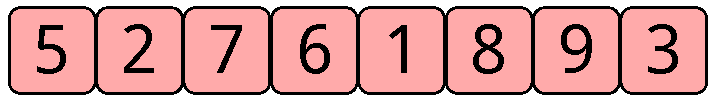
\includegraphics[width=7 cm]{asset/quicksort-concept-1.pdf}
\end{figure}
\end{frame}

\begin{frame}
\frametitle{Konsep (lanj.)}
\begin{itemize}
  \item Tempatkan seluruh elemen yang $\leq 5$ di bagian kiri \farray, dan yang $> 5$ di bagian kanan.
  \item Urutannya elemen setelah pemindahan tidak penting.
\end{itemize}
\begin{figure}
  \centering
  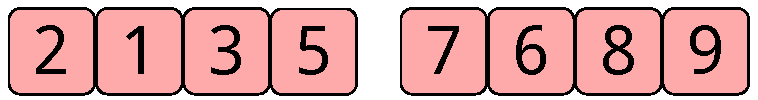
\includegraphics[width=7 cm]{asset/quicksort-concept-2.pdf}
\end{figure}
\end{frame}

\begin{frame}
\frametitle{Konsep (lanj.)}
\begin{itemize}
  \item Lakukan \fQuickSort serupa untuk bagian kiri dan kanan secara rekursif.
  \item Suatu ketika, seluruh \farray menjadi terurut.
\end{itemize}
\begin{figure}
  \centering
  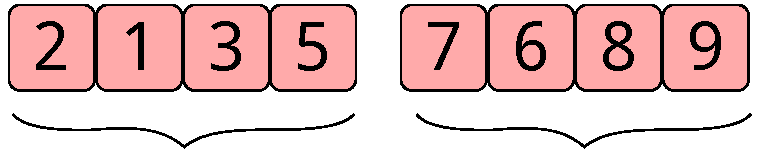
\includegraphics[width=7 cm]{asset/quicksort-concept-3.pdf}
\end{figure}
\end{frame}

\begin{frame}
\frametitle{Konsep (lanj.)}
Jika dikaitkan dengan \fDivideAndConquer:
\begin{itemize}
  \item \foreignTerm{Divide}: partisi \farray menjadi dua seperti yang dijelaskan sebelumnya.
  \item \foreignTerm{Conquer}: ketika \farray tinggal satu elemen, berarti sudah terurut.
  \item \foreignTerm{Combine}: tempelkan hasil \fQuickSort bagian kiri dan kanan.
\end{itemize}
\end{frame}

\begin{frame}
\frametitle{Partisi}
\begin{itemize}
  \item Bagian utama dari \fQuickSort adalah proses partisi (bagian \foreignTerm{divide}).
  \item Sebelum melakukan partisi, pilih suatu elemen yang akan dijadikan \fpivot (=pijakan).
  \item Nantinya, akan dilakukan partisi supaya seluruh elemen yang $\leq pivot$ berada di bagian kiri, dan yang $> pivot$ di bagian kanan.
  \item Untuk saat ini, kita akan menggunakan elemen di tengah \farray $pivot$.
\end{itemize}
\end{frame}

\begin{frame}
\frametitle{Partisi (lanj.)}
\begin{itemize}
  \item Kini sudah ditentukan nilai $pivot$, bagaimana cara mempartisi \farray?
  \item Kita dapat menggunakan sebuah perulangan $O(N)$ untuk menampung hasil partisi di suatu \farray sementara, lalu menempatkan kembali hasil partisi ke \farray sebenarnya.
  \item Namun cara ini agak merepotkan, kita perlu membuat \farray sementara dan memindahkan isi \farray.
\end{itemize}
\end{frame}

\begin{frame}
\frametitle{Partisi Hoare}
\begin{itemize}
  \item Ada beberapa algoritma untuk melakukan partisi secara \foreignTerm{in place}, yaitu tanpa \farray sementara.
  \item Kita akan menggunakan salah satunya, yaitu algoritma partisi \newTerm{Hoare}.
\end{itemize}
\end{frame}

\begin{frame}
\frametitle{Partisi Hoare (lanj.)}
Misalkan $pivot = 5$.

Mulai dengan dua variabel penunjuk, $kiri$ dan $kanan$ di ujung-ujung \farray.
\begin{figure}
  \centering
  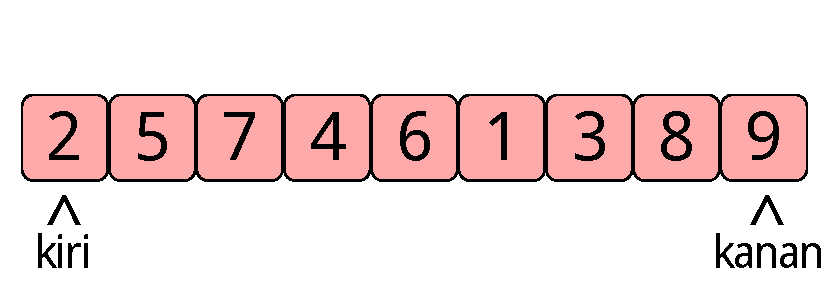
\includegraphics[width=7 cm]{asset/partition-1.pdf}
\end{figure}
\end{frame}

\begin{frame}
\frametitle{Partisi Hoare (lanj.)}
Gerakkan variabel $kiri$ ke arah kanan, sampai elemen yang ditunjuk tidak $< pivot$
\begin{figure}
  \centering
  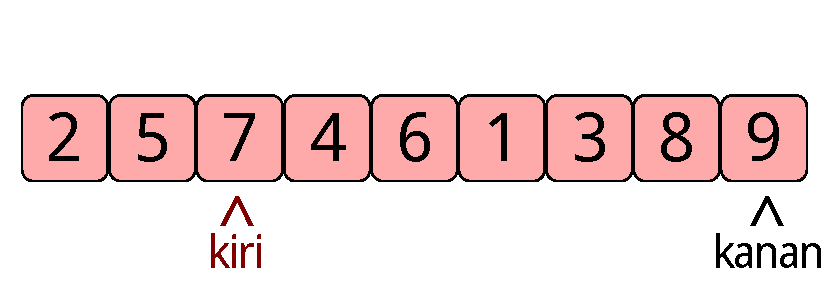
\includegraphics[width=7 cm]{asset/partition-2.pdf}
\end{figure}
\end{frame}

\begin{frame}
\frametitle{Partisi Hoare (lanj.)}
Gerakkan variabel $kanan$ ke arah kiri, sampai elemen yang ditunjuk tidak $> pivot$
\begin{figure}
  \centering
  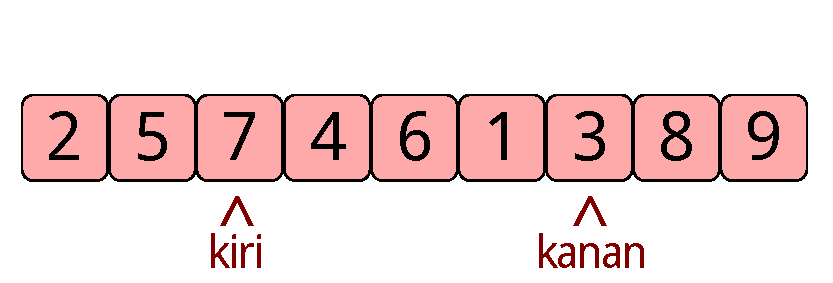
\includegraphics[width=7 cm]{asset/partition-3.pdf}
\end{figure}
\end{frame}

\begin{frame}
\frametitle{Partisi Hoare (lanj.)}
Tukar elemen yang ditunjuk $kiri$ dan $kanan$, lalu gerakkan:
\begin{itemize}
  \item $kiri$ ke kanan satu langkah
  \item $kanan$ ke kiri satu langkah
\end{itemize}
\begin{figure}
  \centering
  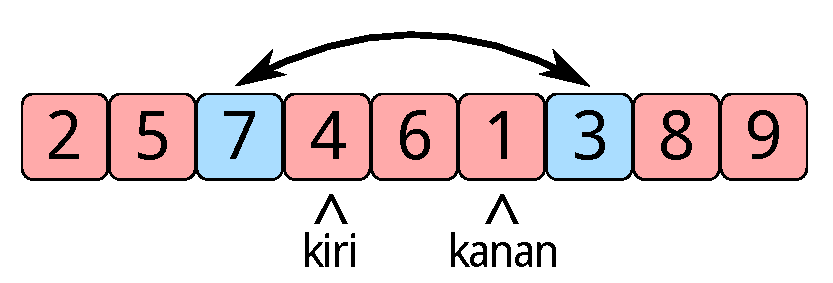
\includegraphics[width=7 cm]{asset/partition-4.pdf}
\end{figure}
\end{frame}

\begin{frame}
\frametitle{Partisi Hoare (lanj.)}
Karena $kiri \leq kanan$, artinya partisi belum selesai.

Kita akan mengulangi hal yang serupa.
\begin{figure}
  \centering
  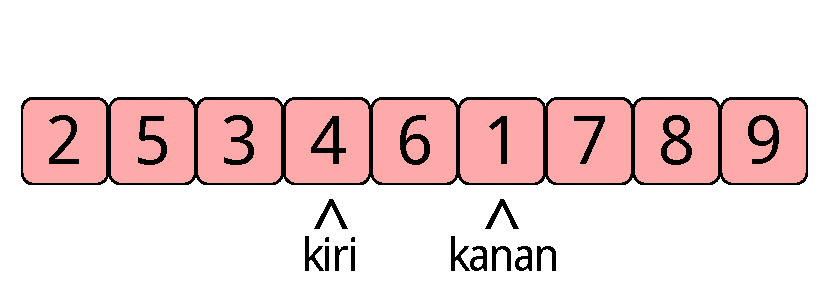
\includegraphics[width=7 cm]{asset/partition-5.pdf}
\end{figure}
\end{frame}

\begin{frame}
\frametitle{Partisi Hoare (lanj.)}
Gerakkan variabel $kiri$.
\begin{figure}
  \centering
  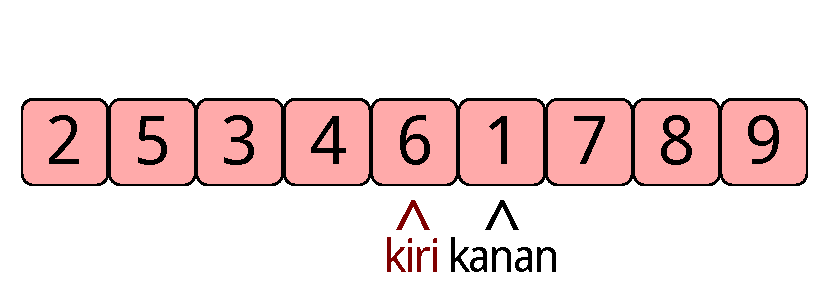
\includegraphics[width=7 cm]{asset/partition-6.pdf}
\end{figure}
\end{frame}

\begin{frame}
\frametitle{Partisi Hoare (lanj.)}
Gerakkan variabel $kanan$.

Kebetulan, elemen yang ditunjuk sudah tidak $> pivot$.
\begin{figure}
  \centering
  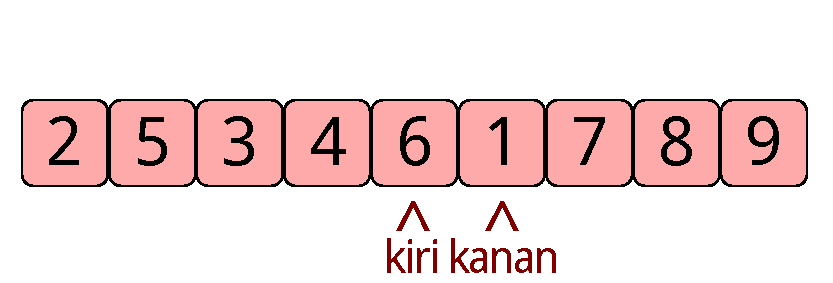
\includegraphics[width=7 cm]{asset/partition-7.pdf}
\end{figure}
\end{frame}

\begin{frame}
\frametitle{Partisi Hoare (lanj.)}
Tukar dan gerakkan variabel $kiri$ dan $kanan$ satu langkah.
\begin{figure}
  \centering
  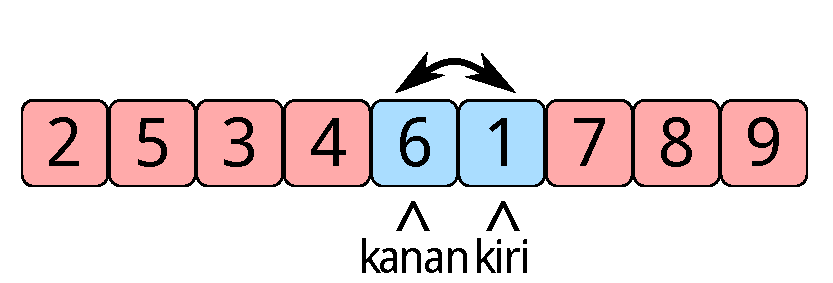
\includegraphics[width=7 cm]{asset/partition-8.pdf}
\end{figure}
\end{frame}

\begin{frame}
\frametitle{Partisi Hoare (lanj.)}
Kini sudah tidak $kiri \leq kanan$, artinya partisi selesai.
\begin{figure}
  \centering
  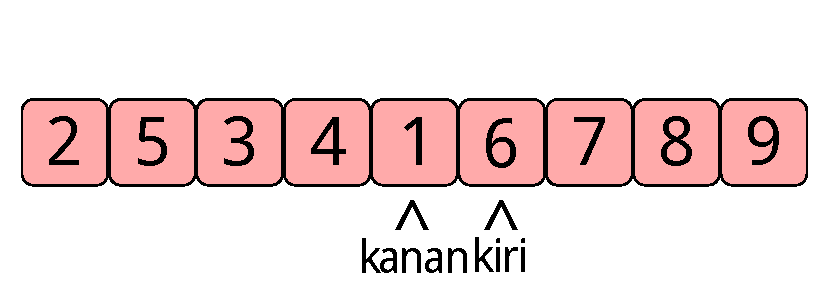
\includegraphics[width=7 cm]{asset/partition-9.pdf}
\end{figure}
\end{frame}

\begin{frame}
\frametitle{Partisi Hoare (lanj.)}
Perhatikan bahwa seluruh elemen yang $\leq pivot$ berada di kiri, dan sisanya di kanan.
\begin{figure}
  \centering
  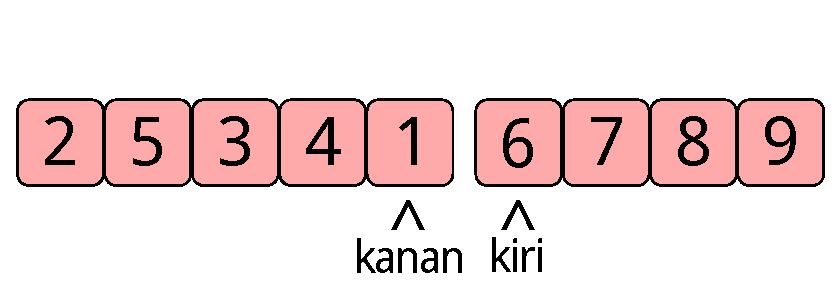
\includegraphics[width=7 cm]{asset/partition-10.pdf}
\end{figure}
\end{frame}

\begin{frame}
\frametitle{Implementasi Partisi Hoare }
\begin{codebox}
\Procname{$\proc{partition}(arr[], left, right, pivot)$}
\li $pLeft \gets left$
\li $pRight \gets right$
\li \While $pLeft \leq pRight$ \Do
\li   \While $arr[pLeft] < pivot$ \Do
\li     $pLeft \gets pLeft + 1$
      \End
\li   \While $arr[pRight] > pivot$ \Do
\li     $pRight \gets pRight - 1$
      \End
\li   \If $pLeft \leq pRight$ \Then
\li     $\func{swap}(arr[pLeft], arr[pRight])$
\li     $pLeft \gets pLeft + 1$
\li     $pRight \gets pRight - 1$
      \End      
    \End
\end{codebox}
\end{frame}

\begin{frame}
\frametitle{Analisis Algoritma Partisi Hoare}
\begin{itemize}
  \item Terdapat dua variabel penunjuk, yang setiap langkahnya selalu bergerak ke satu arah tanpa pernah mundur.
  \item Algoritma berhenti ketika variabel $kiri$ dan $kanan$ bertemu.
  \item Artinya, setiap elemen \farray dikunjungi tepat satu kali.
  \item Kompleksitasnya adalah $O(N)$.
\end{itemize}
\end{frame}

\begin{frame}
\frametitle{Integrasi ke Quicksort}
Setelah kita mengimplementasikan algoritma partisi, mengintegrasikan ke \fQuickSort cukup mudah.
\begin{codebox}
\Procname{$\proc{quicksort}(arr[], left, right)$}
\li \If $left \geq right$ \Then 
\li   \Comment Tidak ada elemen yang perlu diurutkan
\li \Else
\li    $pivot \gets arr[(left + right)$ div $2]$
\zi
\li    \Comment ... sisipkan isi algoritma Hoare di sini ...
\li    \Comment Sampai saat ini, dipastikan $pRight < pLeft$
\zi
\li    $\proc{quicksort}(left, pRight)$
\li    $\proc{quicksort}(pLeft, right)$
    \End
\end{codebox}
\end{frame}

\begin{frame}
\frametitle{Analisis Algoritma Quicksort}
\begin{itemize}
  \item Pada setiap kedalaman rekursif, \farray hasil partisi belum tentu memiliki ukuran yang sama.
  \item Hasil partisi bergantung pada nilai \emp{pivot} yang kita pilih.
  \item Kita anggap dulu hasil partisi selalu membelah \farray menjadi dua \fsubarray sama besar.
\end{itemize}
\end{frame}

\begin{frame}
\frametitle{Analisis Algoritma Quicksort (lanj.)}
\begin{itemize}
  \item Ternyata kejadiannya menjadi seperti \fMergeSort.
  \item Kompleksitasnya adalah $O(N \log{N})$
\end{itemize}

\end{frame}

\begin{frame}
\frametitle{Analisis Algoritma Quicksort: Best Case}
\begin{itemize}
  \item Pembelahan menjadi dua \fsubarray sama besar menjamin kedalaman rekursif \emp{sedangkal mungkin}.
  \item Sehingga untuk kasus terbaik, jalannya algoritma menjadi seperti \fMergeSort dan bekerja dalam $O(N \log{N})$.
\end{itemize}
\begin{figure}
  \centering
  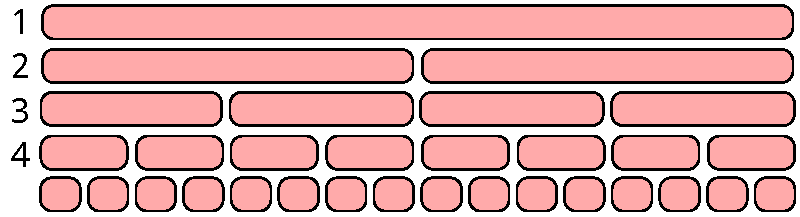
\includegraphics[width=10 cm]{asset/merge-sort-complexity.pdf}
\end{figure}
\end{frame}
  
\begin{frame}
\frametitle{Analisis Algoritma Quicksort: Average Case}
\begin{itemize}
  \item Pada kebanyakan kasus, ukuran hasil partisi berbeda.
  \item Secara rata-rata kompleksitasnya masih dapat dianggap $O(N \log{N})$.
\end{itemize}
\begin{figure}
  \centering
  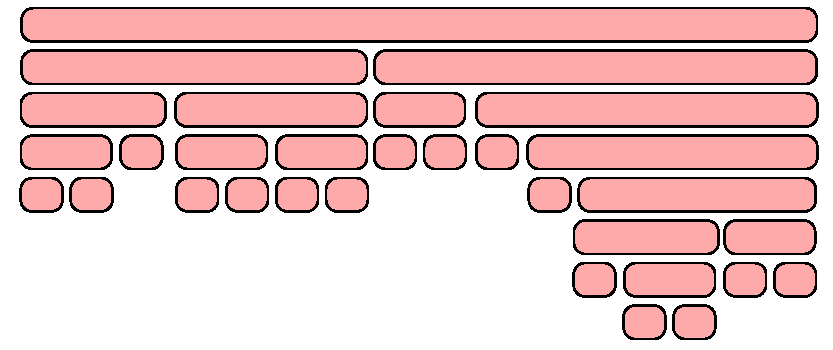
\includegraphics[width=10 cm]{asset/quicksort-complexity-average.pdf}
\end{figure}
\end{frame}

\begin{frame}
\frametitle{Analisis Algoritma Quicksort: Worst Case}
\begin{itemize}
  \item Kasus paling buruk, ukuran hasil partisi sangat timpang.
  \item Akibatnya, kedalaman rekursif mendekati $N$.
  \item Kompleksitasnya menjadi $O(N^2)$.
\end{itemize}
\begin{figure}
  \centering
  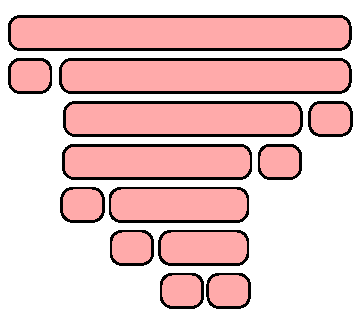
\includegraphics[width=5 cm]{asset/quicksort-complexity-worst.pdf}
\end{figure}
\end{frame}

\begin{frame}
\frametitle{Analisis Algoritma Quicksort (lanj.)}
\begin{itemize}
  \item Tidak perlu khawatir, peluang terjadinya kasus terburuk sangat-sangat-amat-lah  kecil.
  \item Artinya, dijamin 99,9999\% bahwa \fQuickSort akan berjalan dengan sangat cepat.
\end{itemize}
\end{frame}

\begin{frame}
\frametitle{Pemilihan Pivot}
Terdapat beberapa strategi pemilihan $pivot$ untuk mencegah hasil partisi yang terlalu timpang:
\begin{itemize}
  \item Pilih salah satu elemen secara acak, ketimbang selalu memilih elemen di tengah.
  \item Pilih median dari elemen paling depan, tengah, dan paling belakang.
  \newline
\end{itemize}
Cara pertama umum digunakan pada kontes pemrograman rutin seperti \textcolor{blue}{\href{http://codeforces.com/}{Codeforces}}.
\end{frame}

\begin{frame}
\frametitle{Stable Sort}
\begin{itemize}
  \item \fQuickSort memiliki sifat \emp{tidak} \foreignTerm{stable}.
  \item Artinya jika dua elemen $a_1$ dan $a_2$:
  \begin{itemize}
    \item memiliki yang nilai sama
    \item sebelum diurutkan $a_1$ terletak sebelum $a_2$
  \end{itemize}
  maka setelah diurutkan \emp{tidak} dijamin $a_1$ tetap terletak sebelum $a_2$.
\end{itemize}
\end{frame}

\begin{frame}
\frametitle{Penutup}
\begin{itemize}
  \item Terdapat jiwa \fDivideAndConquer pada algoritma \fQuickSort.
  \item Kita telah mempelajari algoritma pengurutan yang efisien lainnya.
\end{itemize}
\end{frame}

\end{document}
